\section{Fluxional execution model} \label{section:model}

\subsection{Fluxions}

The fluxional execution model role is to manage and invoke autonomous execution units.
An execution unit accepts only streams as input and output, that is a continuous and infinite sequence of data encapsulated in messages.
We named this execution unit a fluxion.
That is a function, as in functional programming, only dependent from data streams.
It is composed of a unique name, a processing function, and a persisted memory context.

Messages are carried by a distributed messaging system.
They are composed of the name of the recipient fluxion and a body.
At a message reception, the fluxion modifies its context, and sends back messages to downstream fluxions.
The fluxion's execution context is defined as the set of state variables on which the fluxion depends between two executions - that is two messages receptions.

The fluxions form a chain of processing binded by data streams.
All these chains constitute a directed graph, operated by the messaging system.

\subsection{Messaging system}

The messaging system is the core of our fluxional execution model.
It carries messages along streams, and invokes fluxions at a message reception.

A message queue is at the core of this messaging system.
Each message is processed one after the other by invocation of the recipient fluxion.
% Using a message queue allows to execute multiple processing chains fairly and concurrently, without difference in scheduling local messages, or network messages.
The life cycle of a fluxional application is pictured on figure \ref{fig:MesSys}.

\begin{figure}[h!]
  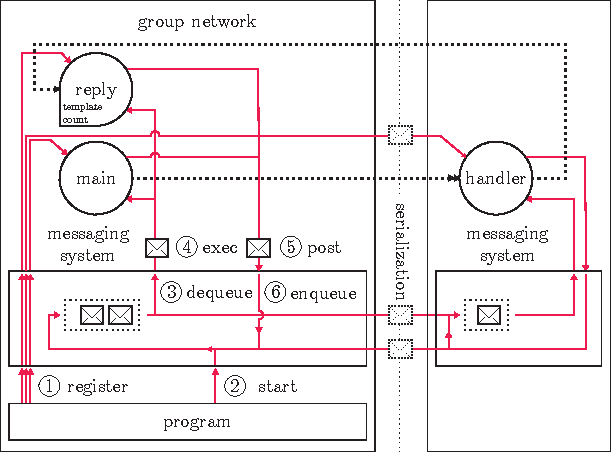
\includegraphics[width=\linewidth]{ressources/schema-message.pdf}
  \caption{Messaging system details}
  \label{fig:MesSys}
\end{figure}

The messaging system carries message streams based on the names of the recipient fluxions.
So it needs every fluxion to be registered.
If two fluxions share a name, the messaging system would be in a conflicting situation.
This registration matches a processing function with a unique name and an initial execution context.
The registration is done using the function \texttt{register(<nom>, <fn>, <context>)}, step \circled{1} on figure \ref{fig:MesSys}.
% A fluxion can dynamically register other fluxions

To trigger a fluxions chain, a message is sent using the function \texttt{start(<msg>)}, step \circled{2}.
This function pushes a first message in the queue.
Immediately, the system dequeues this message to invoke the recipient processing function, step \circled{3} and \circled{4}.
The recipient function sends back messages using the function \texttt{post(<msg>)}, step \circled{5}, to be enqueued in the system, step \circled{6}.
The system loops through steps \circled{3} and \circled{4} until the queue is empty.
This cycle start again for each new start.

The algorithms \ref{alg:traitement} and \ref{alg:parcours} precisely describe the behavior of the messaging system after the function \texttt{start} invocation.

\begin{algorithm}
\caption{Message queue walking algorithm}
\label{alg:parcours}
\begin{algorithmic}
\Function{loopMessage}{\null}
\While{$msg$ \textbf{presents in} $msgQueue$}
\State $msg \gets$ \Call{dequeue}{\null} \Comment{\circled{3}}
\State \Call{ProcessMsg}{$msg$}
\EndWhile
\EndFunction
\end{algorithmic}
\end{algorithm}

\begin{algorithm}
\caption{Message processing algorithm}
\label{alg:traitement}
\begin{algorithmic}
\Function{processMsg}{$msg$}
\For{$dest$ \textbf{in} $msg.dest$}
\State $fluxion \gets lookup(dest)$
\State $message \gets$ \Call{exec}{$fluxion, msg.body$} \Comment{\circled{4} \& \circled{5}}
\State \Call{enqueue}{$message$} \Comment{\circled{6}}
\EndFor
\EndFunction
\end{algorithmic}
\end{algorithm}

\subsection{External interfaces}

In order to interact with other systems, we define external border interfaces.
As a first approach, our goal is to interface Web architectures, so we need to communicate with a REST\cite{Fielding2002} client.
We define two components in this interface :

\begin{itemize}
	\item[\textbf{In}]
    receives client connections.
    % This is so the first link in the chain.
    For every incoming connection, it relays a connection identifier to the \textbf{Out} component for the reply.
    It then relays the connection identifier and the request to the first fluxion by calling the \texttt{start} function.
	\item[\textbf{Out}]
    sends the result of the processing chain back to the client.
    To receive messages from the processing chain, the component \textbf{Out} is registered in the messaging system under the name \texttt{out}.
    % This is so the last link in the chain.
\end{itemize}

Figure \ref{fig:schemaweb} pictures the specific elements of the web interface inside the fluxional system.
% La figure \ref{fig:schemaweb} illustre les éléments spécifiques de cette interface Web au sein du système fluxional illustré par la figure \ref{fig:MesSys}.

\begin{figure}[h!]
	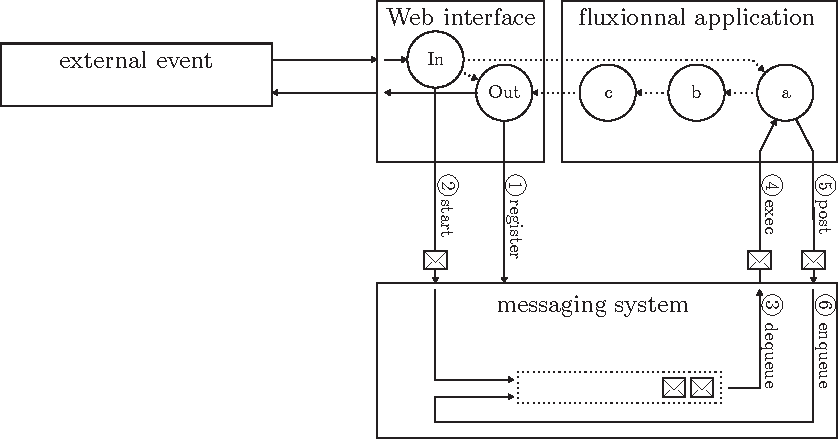
\includegraphics[width=\linewidth]{ressources/schema-web.pdf}
	\caption{Fluxional application with web interface}
	\label{fig:schemaweb}
\end{figure}

% TODO paragraphe de transition

\subsection{Service example}

In order to picture the fluxional execution model, we present an example of a simple visit counting service.
This service counts the number of HTTP connections for each user, and sends him back this number in the HTTP reply.
This example is not a compilation result, but only an illustration for the fluxionnal execution model.

\begin{code}[Javascript, caption={Original code of a simple service example},label={lst:classique}]
var app = require('express')();

@\label{lst:classique_count}@var count = {};

@\label{lst:classique_get}\label{lst:classique_replyb}@app.get('/:id', function reply(req, res){
  count[req.params.id] = count[req.params.id]  || 1; @\label{lst:classique_dynres}@
  ++count[req.params.id] 
  var visits = count[req.params.id];
  var reply = req.params.id + ' connected ' + visits + ' times.';
@\label{lst:classique_send}@  res.send(reply);
@\label{lst:classique_replye}@});

port = 8080;
app.listen(port);
console.log("Listening port: "+port);
\end{code}

The initial version of this service could look like code listing \ref{lst:classique}.
In this code listing, three elements are worth noticing.

\begin{itemize}
  \item The \texttt{count} object at line \ref{lst:classique_count} is a persistent memory that stores each user visit count.
  This object is mapped to a fluxion \textit{execution context} in the fluxional system.
  \item The \texttt{reply} function, line \ref{lst:classique_replyb} to \ref{lst:classique_replye}, contains the logic we want to express in the fluxional processing chain.
  \item The two functions \texttt{get} and \texttt{send}, respectively line \ref{lst:classique_get} and \ref{lst:classique_send}, interface the logic with the external interface.
  The hidden processing chain of functions is : $\texttt{get} \to \texttt{reply} \to \texttt{send}$
\end{itemize}

This minimal service is transformed manually into the fluxions chain depicted in Figure \ref{fig:fluxions}.
We expect a similar result with the compiler described in next section.

\begin{figure}[h!]
  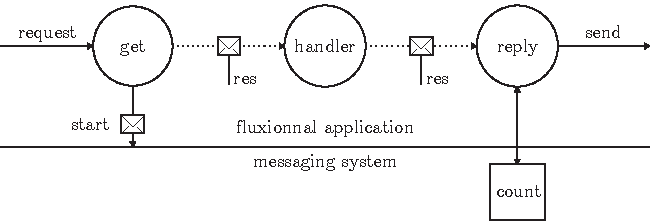
\includegraphics[width=\linewidth]{ressources/flux.pdf}
  \caption{Count service fluxions chain}
  \label{fig:fluxions}
\end{figure}

The circles in figure \ref{fig:fluxions} represent registered fluxions.
Envelope symbols represent exchanged messages between fluxions with the data transmitted from one fluxion to the other. Finally, squares stored in the messaging system hold the \textit{execution context} for the logic and \textbf{Out} fluxions.
When a new \texttt{get} REST message is received at the \textbf{In} end point, a \texttt{start} message triggers the flow.
Concurrently the \textbf{In} fluxion set a \texttt{cid} parameter to the \textbf{Out} fluxion execution context.
This \texttt{cid} is associated to the client connexion to which the last fluxion redirects the answer.
The \texttt{cid} tags the request and is transmitted through the flow until the \textbf{Out} fluxion.
Each fluxion propagates the necessary values from one fluxion to the other exclusively by messages.
Horizontal dashed lines show message virtual transmission between fluxions although they all go through the messaging system.

Listing \ref{lst:fluxional} describes this counting service in our fluxional language.
This new language brings a stricter segmentation than the initial code by allowing the developer to only define and register fluxions.
% And so, it allows an additional system to optimize the organization of the system on different physical machines according to the cost of fluxions' streams and processing.
A fluxion is defined by a name, and a list of destinations preceded by the operator \texttt{-}\texttt{>}.
Fluxions can access and manipulate only two objects : \texttt{msg} and \texttt{this}.
The first is the received message, the second is the persisted context of the fluxion.
Fluxions use the Javascript language syntax inside their definition.

% This high level language is not dynamic, and not typed.
% You can register fluxion at any time, and the messages can contain any type or composition of types.
% \TODO{write a paragraph about the languages characteristics, a reserved subsection might be necessary, but maybe better placed in the next section, about transformation}

\begin{code}[Javascript, caption={Fluxional sample},label={lst:fluxional}]
use web

fluxion logic -> view
  this.uid[msg.uid] = this.uid[msg.uid] + 1 || 1
  msg.count = this.uid[msg.uid]
  post msg

fluxion view -> output
  msg.view = msg.uid + " connected " + msg.count + " times."
  msg.uid = undefined
  msg.count = undefined
  post msg

register logic, {uid: {}}
register view

web.listen
\end{code}

Except from the two interface components, the service is organized as follow :
\begin{itemize}
  \item The \texttt{logic} fluxion is the first to receive the client's message.
  It contains the whole logic of this simple service.
  A real service would need a more complex chain with logic distributed across multiple fluxions, instead of a single fluxion.
  It increments the count for the received user identifier, pushes this count inside the message, and relays it to the next fluxion.
  \item The \texttt{view} fluxion receives this message, formats it for the user, and relays it to the output fluxion.
\end{itemize}

We use this interface to develop web services using the fluxional execution model.
But our goal, as described in the introduction, is to automate this architecture shift, not to impose a new programming paradigm onto the developer.
% We now evaluate this model against the basic one.


